% Chapter 1

\chapter{Introducción general} % Main chapter title

\label{Chapter1} % For referencing the chapter elsewhere, use \ref{Chapter1} 
\label{IntroGeneral}

%----------------------------------------------------------------------------------------

% Define some commands to keep the formatting separated from the content 
\newcommand{\keyword}[1]{\textbf{#1}}
\newcommand{\tabhead}[1]{\textbf{#1}}
\newcommand{\code}[1]{\texttt{#1}}
\newcommand{\file}[1]{\texttt{\bfseries#1}}
\newcommand{\option}[1]{\texttt{\itshape#1}}
\newcommand{\grados}{$^{\circ}$}

%----------------------------------------------------------------------------------------

%\section{Introducción}


%----------------------------------------------------------------------------------------

En este capítulo se presentan los conceptos básicos de la diálisis renal. Además se mencionan las motivaciones que impulsan este trabajo de investigación, se establecen los objetivos, el alcance y los requerimientos, y se revisa el estado del arte en el campo de estudio.

\section{Conceptos básicos de la diálisis renal}

En esta sección se abordan las definiciones de diálisis renal y sus principales tipos de tratamientos.

\subsection{Diálisis renal y tipos de tratamiento}

La diálisis renal es un tratamiento en el que se extraen las toxinas y el exceso de agua de la sangre. Se utiliza como terapia renal sustitutiva cuando los riñones no funcionan correctamente debido a su deterioro. Los riñones desempeñan un papel crucial al eliminar las toxinas y el líquido de la sangre, evitando que los productos de desecho se acumulen en el cuerpo. Cuando los riñones no pueden realizar esta función, la diálisis se convierte en una herramienta vital.

Existen dos tipos principales de tratamientos de diálisis renal \citep{ARTICULO1}:

\begin{itemize}
\item Hemodiálisis (HD): En este tratamiento se utiliza una membrana artificial. La purificación de la sangre se lleva a cabo mediante un riñón artificial, que elimina el exceso de agua, residuos y toxinas antes de devolverla al cuerpo. Cada sesión de hemodiálisis puede durar aproximadamente cuatro horas y debe realizarse unas tres veces por semana.
\item Diálisis Peritoneal (DP): En este método de tratamiento, la filtración de la sangre se realiza en la cavidad peritoneal del paciente. Se utiliza un catéter permanente que se coloca en el abdomen, a través del cual se introduce una solución especial llamada líquido de diálisis en la cavidad peritoneal. Esta solución absorbe los desechos y el exceso de líquido del cuerpo a través de la membrana peritoneal, que actúa como una barrera semipermeable. Luego, después de un período de tiempo especificado (generalmente varias horas), el líquido de diálisis se drena del abdomen, llevando consigo los desechos y el exceso de líquido. Hay dos variantes de diálisis peritoneal: 
    \begin{itemize}
    \item Diálisis Peritoneal Continua Ambulatoria (DPCA): El paciente realiza los intercambios de líquido de diálisis manualmente varias veces al día, mientras sigue con sus actividades diarias. No se requiere una máquina para realizar los intercambios y el proceso es llevado a cabo por el paciente o su cuidador.
    \item Diálisis Peritoneal Automática (DPA): En este método, se utiliza una máquina cicladora para realizar los intercambios de líquido de diálisis durante la noche mientras el paciente duerme. La máquina administra automáticamente el líquido de diálisis, lo retira y lo reemplaza según un programa preestablecido. Esto permite una mayor flexibilidad en el tratamiento y puede ser más conveniente para algunos pacientes.
    \end{itemize}
\end{itemize}

En la figura \ref{fig:diagDialisis} se muestra la diferencia entre ambos tratamientos.

\begin{figure}[htpb]
\centering 
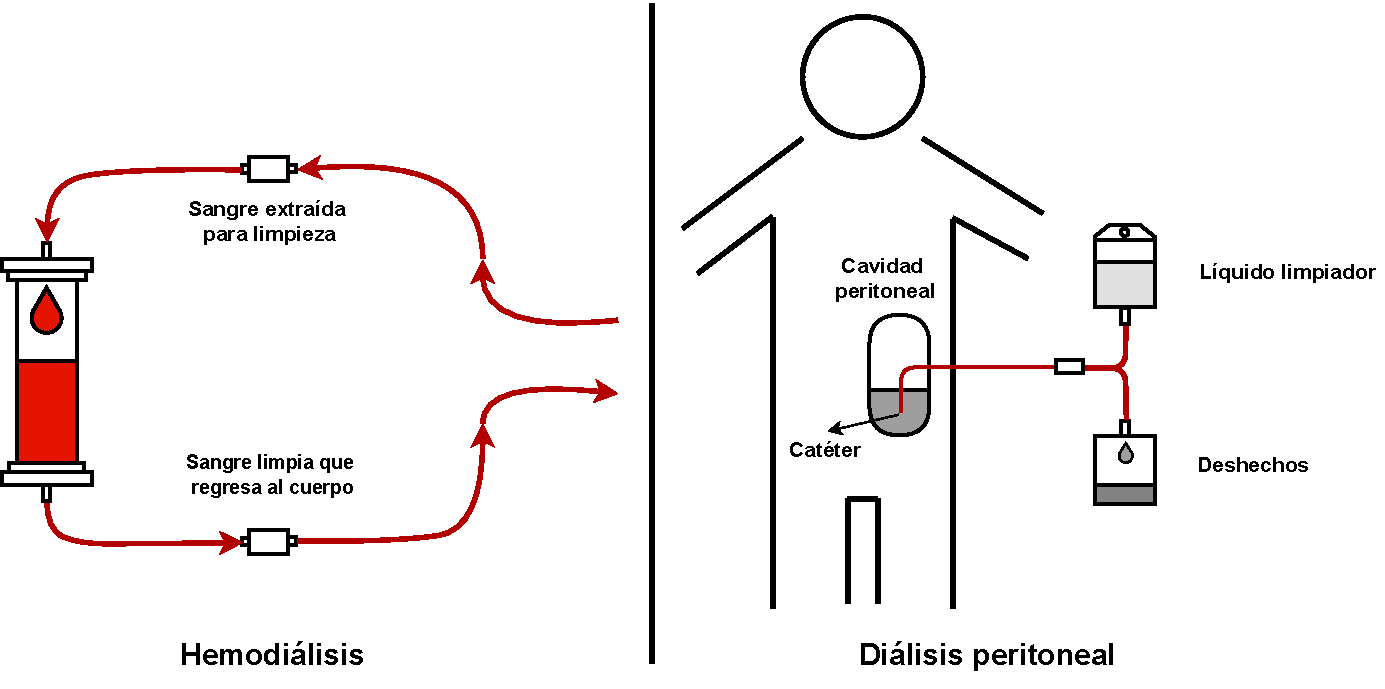
\includegraphics[width=.95\textwidth]{./Figures/Dialisis.pdf}
\caption{Diferencia entre hemodiálisis y diálisis peritoneal.}
\label{fig:diagDialisis}
\end{figure}


\section{Contexto y motivación}

La motivación principal de este trabajo es incorporar técnicas de inteligencia artificial (IA) en el campo de la medicina, dado que han demostrado una notable capacidad para anticipar eventos futuros basándose en datos históricos \citep{ARTICULO2}. 
Pero uno de los desafíos recurrentes a la hora de entrenar modelos de IA es la obtención de datos representativos. En el ámbito de la medicina este desafío también se hace presente, ya que se suele contar con pocos datos médicos de una población muy reducida.
Para el desarrollo de este trabajo se contó con datos médicos de unos catorce mi pacientes que estuvieron bajo tratamiento de diálisis renal. 
Tanto el equipo de sistemas como el equipo médico de ésta empresa de diálisis renal, si bien no tienen experiencias en herramientas de IA para predicción de eventos, conocen el potencial de estos modelos para identificar patrones, por lo que colaboraron en el desarrollo de este trabajo para lograr el cumplimiento del objetivo.

%----------------------------------------------------------------------------------------

\section{Objetivos, alcance y requerimientos}

\subsection{Objetivos}

El propósito de este trabajo fue el desarrollo de un modelo de IA que permite predecir el riesgo de mortalidad en pacientes en diálisis renal, junto con la configuración de una plataforma de administración de modelos, una interfaz de comunicación con el modelo y un proceso que solicite las predicciones continuamente. Este conjunto de herramientas provee una predicción actualizada del riego de mortalidad de los pacientes, lo que permite al personal médico adaptar el tratamiento y la medicación prescrita para mejorarles su calidad de vida y, en última instancia, salvar vidas. En la figura \ref{fig:diagArqBasic} se muestra la arquitectura de la solución propuesta. 

\begin{figure}[htpb]
\centering 
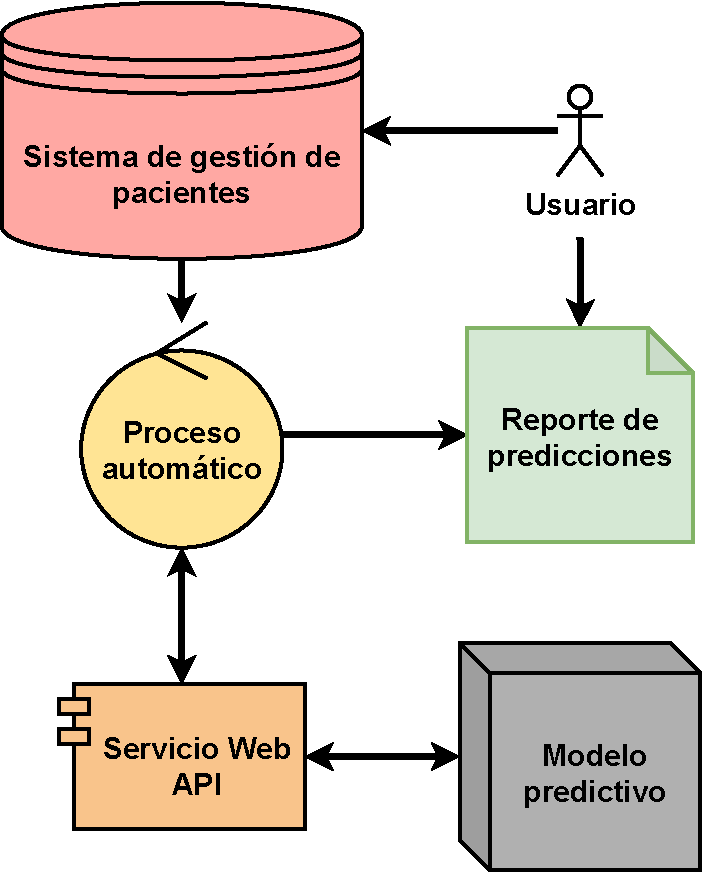
\includegraphics[width=.50\textwidth]{./Figures/Arquiectura_Solucion_Basica.pdf}
\caption{Arquitectura de solución.}
\label{fig:diagArqBasic}
\end{figure}


\subsection{Alcance}

Se encuentra dentro del alcance del trabajo la instalación y configuración de una plataforma de gestión de modelos que permite desplegar modelos en distintos ambientes, el desarrollo de un modelo de predicción de mortalidad, y la construcción de una interfaz y un proceso automático que actúan como nexo entre el modelo predictivo y el sistema de gestión de pacientes.
Para el desarrollo del modelo, se elabora un conjunto de datos con variables médicas de pacientes en diálisis renal. El conjunto de datos debe estar en cumplimiento con la ley 25.326 para garantizar el derecho al honor y a la intimidad de los pacientes en cuestión. Asimismo, se incluye en el alcance el pre-procesamiento del conjunto de datos y el análisis de las distintas métricas para evaluar el correcto desempeño del modelo.

Sin embargo, no se encuentra dentro del alcance del proyecto el desarrollo de una plataforma de gestión, sino que se eligió una existente que cumple con los requerimientos del trabajo, ni el desarrollo de una interfaz web orientada al usuario final. Tampoco se encuentra dentro del alcance la instalación del modelo predictivo en el entorno productivo de la empresa médica. Lo único que se instala en el entorno de la empresa médica será el proceso que recupera datos de los pacientes y llama al servicio web cada cierto período de tiempo para recuperar las predicciones. 

\subsection{Requerimientos}
A continuación, se listan los requerimientos principales del trabajo agrupados por afinidad:
\begin{enumerate}
	\item Requerimientos funcionales
		\begin{enumerate}
			\item La plataforma de gestión de modelos deberá permitir desplegar modelos en diversos ambientes.
			\item La interfaz por servicio web deberá recibir datos médicos de uno o varios pacientes y devolver las predicciones asociadas a ellos.			
			\item El modelo predictivo deberá tener una precisión de al menos un 75\%.
			\item El proceso que solicita predicciones y genera el reporte al usuario deberá poder ejecutarse automáticamente cada cierto período de tiempo.		
			\item El reporte de predicciones que le llegue al usuario final deberá tener un formato claro y comprensible.
			\item Se utilizará GIT como repositorio para el control de version de código
		\end{enumerate}
	\item Requerimientos de datos a utilizar
		\begin{enumerate}		
		\item Durante el entrenamiento del modelo se deberá resguardar la confidencialidad de los datos de los pacientes.		
		\end{enumerate}
	\item Requerimientos de documentación
		\begin{enumerate}
			\item Redactar una memoria técnica con la información del proyecto.
			\item La documentación de la interfaz por servicio web deberá incluir la lista de métodos disponibles con su detalle.
			\item La documentación del modelo predictivo incluirá información sobre el origen de los datos utilizados para el entrenamiento, las características que se usaron, el detalle del modelo seleccionado y la información que haya sobre la explicabilidad del modelo.
		\end{enumerate}		
\end{enumerate}

%----------------------------------------------------------------------------------------

\section{Estado del arte}

Se llevó a cabo una exhaustiva revisión de la literatura relacionada con la predicción de la mortalidad de pacientes en diálisis renal y se ha encontrado principalmente una tesis doctoral \citep{ARTICULO3} muy relevante que plantea un objetivo similar pero cuenta con muchos menos datos para el entrenamiento de los modelos. Si bien las variables médicas seleccionadas para realizar las predicciones en dicha tesis son muy similares a las que se seleccionaron en este trabajo, allí se plantea la discriminación de los casos según el tiempo que los pacientes llevan en diálisis, ya sea tres meses, seis meses, un año o más. Los modelos utilizados en dicha tesis incluyen Bósque Aleatorio (\textit{Random Forest}) y Regresión Logística, algunos de los cuales también fueron utilizados en este trabajo.
En cuanto a las conclusiones, para evaluar el desempeño de los modelos se utilizó la métrica de Área bajo la curva (AUC), la cual llega a valores entre 70\% y 73\%.
En esta tesis también se muestra qué variables tienen mas influencia al realizar la predicción de mortalidad del paciente, lo que resulta sumamente importante para el personal médico.
También se ha encontrado una investigación \citep{ARTICULO4} donde se utilizan técnicas de IA para predecir la mortalidad en pacientes con enfermedad renal crónica. La misma también cuenta con muy pocos datos de pacientes en diáfisis renal y, aunque no se da mucho detalle sobre el entrenamiento de los modelos, concluye indicando que con un modelo de red neuronal se obtiene una predicción superior al 90\%, mejor que con una Regresión Logística.
Por otro lado, se ha encontrado otra tesis \citep{ARTICULO5} orientada comprobar si el índice neutrófilo/linfocito es un predictor de mortalidad en pacientes que inician hemodiálisis. Si bien no se entrena ningún modelo de IA en la investigación, se concluye en que dicho índice no es un predictor de la mortalidad pero que la edad mayor a 60 años si representa un factor de riesgo. 
Existen muchos otros trabajos relacionados con la temática de la predicción de mortalidad en pacientes con enfermedades renales, donde algunos abordan el beneficio que aporta la IA en la detección y predicción de eventos en medicina \citep{ARTICULO6}\citep{ARTICULO7}\citep{ARTICULO9}, otros la predicción de mortalidad teniendo enfermedad renal junto con enfermedad coronaria \citep{ARTICULO10}, y otros la predicción de contraer algún cáncer renal \citep{ARTICULO8}.

Si bien existe literatura académica que aborda el tema de la predicción de mortalidad de pacientes en diálisis renal, la mayoría de los trabajos se centran en investigaciones de carácter teórico y experimental, y además parten de conjuntos de datos muy chicos, lo cual no permite a los modelos generalizar el conocimiento para poder realizar predicciones correctas. Este trabajo se destaca por su enfoque práctico, ya que se desarrolla una herramienta concreta que pueda ser implementada en una empresa médica dedicada a la diálisis renal. Se espera obtener predicciones en tiempo real para los pacientes en diálisis renal y en base a su riesgo de mortalidad adecuar el tratamiento y la medicación prescrita. Esta iniciativa ofrece una solución práctica y viable en el ámbito clínico, lo que contribuye a mejorar la atención y seguimiento de los pacientes.